\documentclass{standalone}
\usepackage{tikz}
\usetikzlibrary{positioning}

\begin{document}
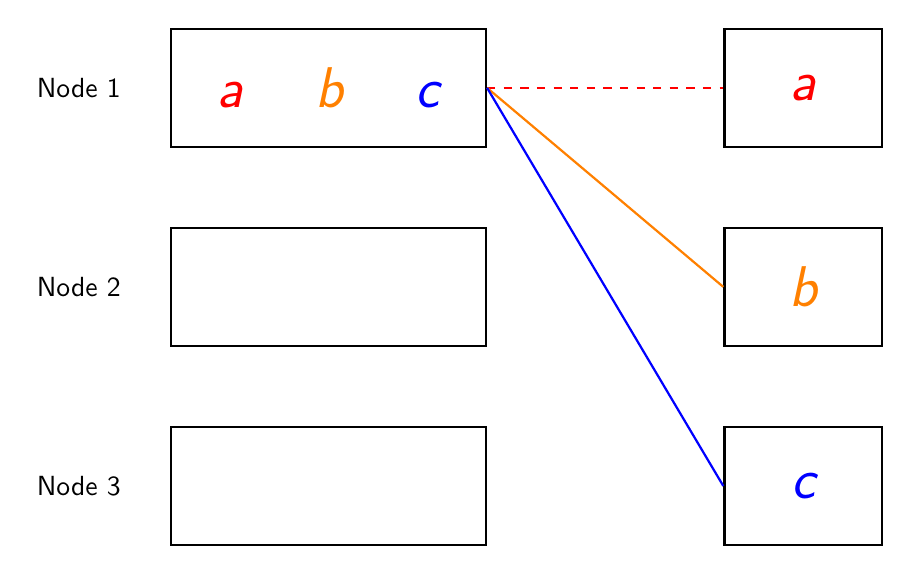
\begin{tikzpicture}[
    node distance=1cm,
    every node/.style={font=\sffamily},
    box/.style={draw, thick, minimum width=2cm, minimum height=1.5cm, align=center},
    longbox/.style={draw, thick, minimum width=4cm, minimum height=1.5cm, align=center}
]

% 左侧节点
\node[longbox] (node1) {\itshape\huge\color{red}a \quad \color{orange}b \quad \color{blue}c};
\node[longbox, below=of node1] (node2) {};
\node[longbox, below=of node2] (node3) {};

% 左侧标签
\node[left=0.5cm of node1] {Node 1};
\node[left=0.5cm of node2] {Node 2};
\node[left=0.5cm of node3] {Node 3};

% 右侧长方形节点
\node[box, right=3cm of node1] (right1) {\itshape\huge\color{red}a};
\node[box, below=of right1] (right2) {\itshape\huge\color{orange}b};
\node[box, below=of right2] (right3) {\itshape\huge\color{blue}c};

% 连接线
% 从node1 (a) 出发的线
\draw[red, thick, dashed] (node1.east) -- (right1.west);
\draw[orange, thick] (node1.east) -- (right2.west);
\draw[blue, thick] (node1.east) -- (right3.west);

\end{tikzpicture}
\end{document}